\documentclass[convert={density=300,size=1080x800,outext=.png}]{standalone}
\usepackage{units}
\usepackage{rotating}
\usepackage{tikz}
\usepackage{pgfplots}
\usepackage{pgfplotstable}
\usepgfplotslibrary{units}
\usetikzlibrary{positioning,calc,fit,automata,chains,patterns,shadows,shapes,backgrounds,shapes.multipart,arrows}

\pgfplotsset{
        tick label style={font=\footnotesize},
        label style={font=\footnotesize},
        legend style={font=\footnotesize},
        legend cell align=left,
	compat=1.10
}

\begin{document}

\pgfplotsset{
    integral segments/.code={\pgfmathsetmacro\integralsegments{#1}},
    integral segments=3,
    integral/.style args={#1:#2}{
        ybar interval,
        domain=#1+((#2-#1)/\integralsegments)/2:#2+((#2-#1)/\integralsegments)/2,
        samples=\integralsegments+1,
        x filter/.code=\pgfmathparse{\pgfmathresult-((#2-#1)/\integralsegments)/2}
    }
}

\centering
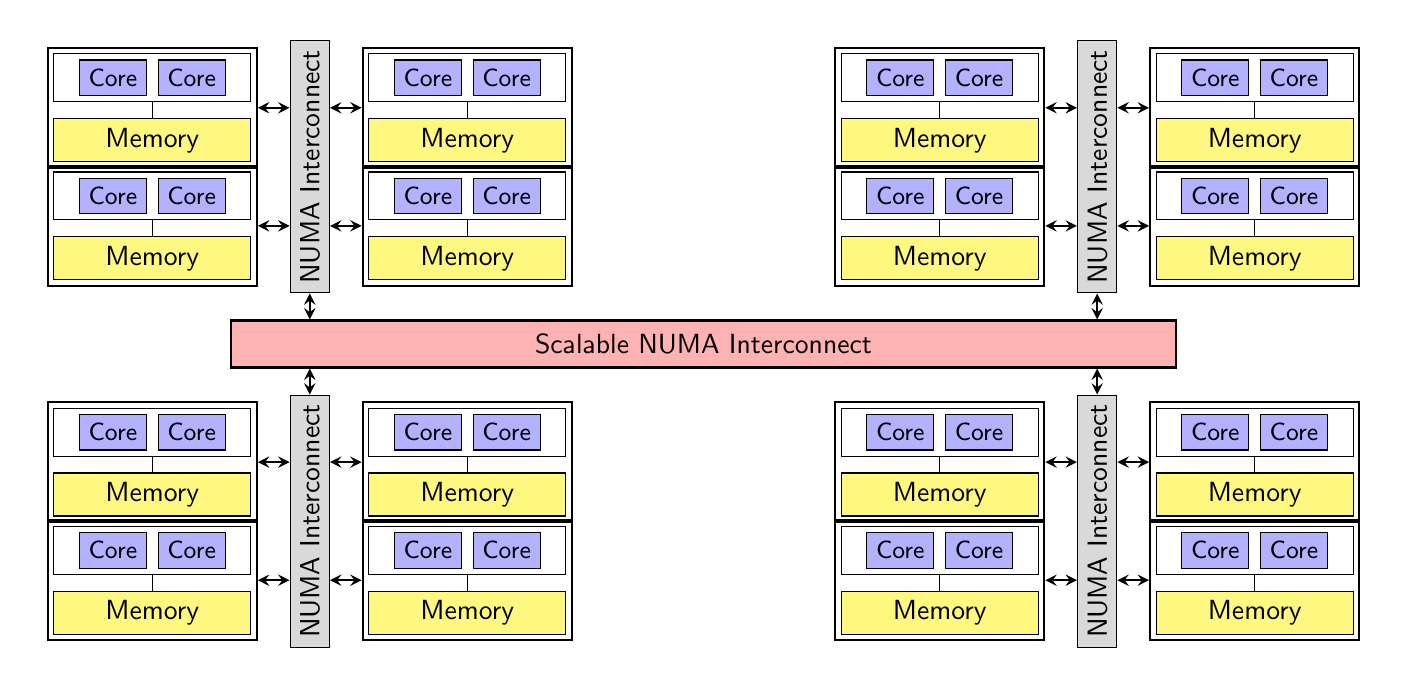
\begin{tikzpicture}[double distance=1pt,every node/.style={font=\sf}]
\foreach \a in {0,1} {
\foreach \b in {0,1} {
\begin{scope}[xshift=10*\a cm,yshift=4.5*\b cm]
\foreach \j in {0,1} {
\foreach \i in {0,1} {
\begin{scope}[xshift=4*\i cm,yshift=1.5*\j cm]
%
\node[draw,rectangle,fill=blue!30] (a){\small Core};
\node[draw,rectangle,fill=blue!30,right of=a] (b){\small Core};
\node[draw,fit = (a) (b),minimum width=2.5cm,inner sep=2pt](c){};
%
\node[draw,rectangle,fill=yellow!50,minimum width=2.5cm,below=.2cm of c](d){Memory};
\draw (c) -- (d);
\node[draw,fit=(c)(d),thick,inner sep=2pt](n\i\j){};
%
\end{scope}
}
}
\node[fit=(n00)(n11)](N\a\b){};
\end{scope}
\node[draw,minimum width=.5cm,fill=gray!30] at (N\a\b.center) (NI\a\b)
{\begin{sideways}NUMA Interconnect\end{sideways}};
%
\foreach \h/\k/\f in {n00/east/west,n01/east/west,n10/west/east,n11/west/east}
{
        \path(\h.\k) -| (NI\a\b.north \f) node[midway](temp){};
        \draw[stealth-stealth,thick] (\h.\k) -- (temp.center);
}
}
}
\begin{pgfonlayer}{background}
\node[fit=(N00)(N11)](SNI){};
\node[draw,thick,fill=red!30,inner sep=5pt,minimum width=12cm] at (SNI) (MI){Scalable NUMA Interconnect};
\end{pgfonlayer}
\foreach \h/\k/\f in {NI00/north/south ,NI10/north/south ,NI01/south/north ,NI11/south/north }
{
        \path (\h.\k) |- (MI.\f east) node[midway](temp){};
        \draw[stealth-stealth,thick] (\h.\k) -- (temp.center);
}
%
%\path (MI) |- (N00)
%node[midway,draw,cloud,aspect=2,fill=gray!20,text width= 1.8cm,align=center,inner sep=1pt,]{Network Interface};
%
%\path (MI) |- (N11)
%node[midway,draw,cylinder,aspect=0.25,shape border rotate=90,fill=blue!30,text width= 2cm,align=center]{Storage Subsystem};
\end{tikzpicture}
\end{document}
